\chapter{KONTINUIRANI RAZVOJ NA PRIMJERU WEB APLIKACIJE}
U prijašnjem su poglavlju opisani programi i infrastruktura potrebna za kontinuirani razvoj
aplikacije. U ovom poglavlju je opisana implementacija sustava za kontinuirani razvoj na primjeru
web aplikacije za izračun fibonaccijevog broja koja je spremljena na Git projektu nazvanom
\textit{diplomski-go}. Opisan je proces izrade aplikacije pomoću Jenkins posla te objavljivanje
aplikacije pomoću servisa za menadžment. Zatim je opisan i proces vraćanje na prethodnu verziju
aplikacije.

\section{Aplikacija za izračun fibonaccijevog broja}
Za testiranje sustava kontinuiranog razvoja izrađen je web program za izračun fibonaccijevog broja
u Go programskom jeziku. Fibonaccijev broj definiran je formulom~\ref{eq:03fibonacci}.

\begin{equation}
    f(n) = \begin{cases}
               0                & n = 0\\
               1                & n = 1\\
               f(n-1) + f(n-2)  & n > 1
           \end{cases}
   \label{eq:03fibonacci}
\end{equation}

U prvoj iteraciji programa koristi se naivno, rekurzivno rješenje vremenske i memorijske
kompleksnosti $O(2^N)$. Prilikom primitka HTTP zahtjeva, program pokreće računanje fibonaccijevog
broja, kao što je prikazano programskim kodom~\ref{03fibv1}.

\lstset{caption={Fibonacci v1}, label=03fibv1}
\begin{lstlisting}[float=h]
func fibonacci(n uint64) uint64 {
	if n == 0 {
		return 0
	} else if n == 1 {
		return 1
	} else {
		return fibonacci(n-1) + fibonacci(n-2)
	}
}
\end{lstlisting}

Funkcija fibonacci prima broj kao parametar. Ukoliko je broj nula, vraća vrijednost nula.
Ukoliko je broj jedan, vraća vrijednost jedan. U protivnom vraća zbroj dvije fibonacci funkcije.
Prva funkcija ima parametar $broj-1$, dok druga funkcija ima broj $broj-2$. Na primjer, ako je
zatražen broj pet, funkcija vraća zbroj dvije fibonacci funkcije, jedna s parametrom četiri, a druge
s tri. Kako bi se provjerila ispravnost koda, napisani su jednostavni testovi jedinice, prikazano
kodom~\ref{03fibunit}

\lstset{caption={Testiranje jedinice}, label=03fibunit}
\begin{lstlisting}[float=h]
func testEqual(t *testing.T, expected, actual uint64) {
	if expected == actual {
		return
	}
	t.Errorf("Greska: \%d (ocekivano) != \%d (dobiveno)", expected, actual)
}

func TestFibonacci(t *testing.T) {
	testEqual(t, uint64(5), fibonacci(5))
	testEqual(t, uint64(8), fibonacci(6))
	testEqual(t, uint64(89), fibonacci(11))
}

\end{lstlisting}

Za sustav testiranja korišten je $testing$ paket koji se nalazi u standardnoj Go biblioteci. Testovi
jedinice se sastoje od jednog testa s tri provjere gdje se provjerava vrijednost petog, šestog i
jedanaestog fibonaccijevog broja.  Unutar svakog testa poziva se pomoćna funkcija koja prima tri
vrijednosti: trenutni test, očekivana vrijednost te dobivena vrijednost. Ukoliko dobivena vrijednost
nije jednaka očekivanoj vrijendosti, funkcija će označiti takav test netočnim.

Za pozivanje fibonacci funkcije kreirana je web aplikacija, kao što je prikazano
slikom~\ref{fig:03fibv1png}. Web aplikacija se sastoji od obrasca koji sadrži prostor za unos teksta
te gumb za izvršavanje operacije. Pritiskom na gumb izvršava se HTTP XHR zahtjev te se po završetku
istoga prikazuje rezultat ili greška ako je do nje došlo.

\begin{figure}[h]
    \centering
    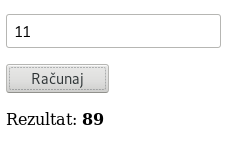
\includegraphics[width=0.3\textwidth]{img/03/fibonacci_html.png}
    \caption{Izgled fibonacci web aplikacije}%
    \label{fig:03fibv1png}
\end{figure}

U glavnoj funkciji koja se poziva prilikom pokretanja programa, \texttt{main}, pokrenut je HTTP
servis zadužen za posluživanje HTTP zahtjeva. Pokretanje HTTP servisa dan je kodom~\ref{03fibhttp}.

\lstset{caption={HTTP servis}, label=03fibhttp}
\begin{lstlisting}[float=h]
func fibonacciHandler(w http.ResponseWriter, r *http.Request) {
	n, err := strconv.ParseUint(r.URL.Query().Get("n"), 10, 64)
	if err != nil {
		w.WriteHeader(http.StatusBadRequest)
		w.Write([]byte("Parametar n mora biti prirodni broj."))
		return
	}
	w.WriteHeader(http.StatusOK)
	w.Write([]byte(strconv.FormatUint(fibonacci(n), 10)))
}

func homePageHandler(w http.ResponseWriter, r *http.Request) {
	http.ServeFile(w, r, "./static/index.html")
}

func main() {
	http.HandleFunc("/", homePageHandler)
	http.HandleFunc("/api/fibonacci", fibonacciHandler)
	log.Fatal(http.ListenAndServe(":8888", nil))
}
\end{lstlisting}

Unutar $main$ funkcije stvorena su dva HTTP rukovoditelja~(\textit{engl.~handlers}). Prvi
rukovoditelj obrađuje zahtjeve za početnu stranicu te, neovisno o bilo kojim argumentima, poslužuje
statičnu datoteku koja se nalazi na lokaciji \texttt{static/index.html}.

Drugi rukovoditelj obrađuje zahtjeve za stranicu \texttt{/api/fibonacci}. Preko GET parametra
očekuje varijablu $n$ te ju pretvara u ne-negativni cijeli broj. Ukoliko program nije u mogućnosti
to napraviti, vraća grešku korisniku. U protivnom poziva fibonacci funkciju s dobivenim brojem te
vraća vrijednost korisniku u tekstualnom obliku.

\textit{End-to-end} testovi prikazani kodom~\ref{03fibe2e} sastoje se od dva testa. Prvi test je
test u kojem se zadaje ispravan argument i zadaje izračun 11.~fibonaccijevog broja. Cypress alat
otvara internet preglednik te otvara zadanu web stranicu. Nakon uspješnog otvaranja u tekstualnu
kućicu unosi broj 11 te pritišće gumb "Računaj". Zatim očekuje da će stranica prikazati broj 89,
koji je traženo rješenje. U drugom testu zatražen je -1.~fibonaccijev broj. Kako to nije moguće
izračunati, očekivanje je da će stranica prikazati grešku da broj mora biti prirodan.

Ukoliko Cypress ne može pronaći traženi element unutar zadanog intervala, takav test je označen kao
neuspješan. Na primjer, ukoliko na stranici ne postoji element s identifikacijom \texttt{number},
test će biti neuspješan. Test će također biti neuspješan ukoliko HTTP XHR zahtjev ne bude uspješan.

Cypress testovi se mogu pokrenuti na lokalnom računalu pomoću naredbe $cypress~open$. Izmjena
testova će automatski biti dostupna unutar grafičkog sučelja Cypress. Testovi se također mogu
pokrenuti naredbom $cypress~run$ koja pokreće testove te izlazi po završetku svih. Rezultati su
dostupni preko standardnog izlaza i izlaznog stanja.

\lstset{caption={\textit{End-to-end} testiranje}, label=03fibe2e}
\begin{lstlisting}[language=php,float=h]
describe('Fibonacci test', function() {
    it("Ispravna forma", function() {
        cy.visit('/');

        cy.get('#number').type('11');
        cy.get('form').contains('Racunaj').click();
        cy.contains('89');
    });

    it("Neispravna forma", function() {
        cy.visit('/');

        cy.get('#number').type("-1");
        cy.get('form').contains('Racunaj').click();
        cy.contains('Parametar n mora biti prirodni broj.');
    });
})
\end{lstlisting}

\section{Jenkins posao za izgradnju i objavu Docker slike}
Za Jenkins posao koji izrađuje Docker sliku i objavljuje u Docker repositorij odabrana je Jenkins
linija. Jenkins linija je isprogramirana i spremljena u datoteci~\texttt{Jenkinsfile} unutar
fibonacci projekta. Jenkins linija se sastoji od šest faza: dohvaćanje koda preko Git projekta,
pokretanje testova jedinica, izgradnja Docker slike, pokretanje \textit{end-to-end} testova,
objava Docker slike u javni Docker repositorij te objava rezultata. Na
slici~\ref{fig:03jenkins_pipeline} prikazana je Jenkins linija.

\begin{figure}[h]
    \centering
    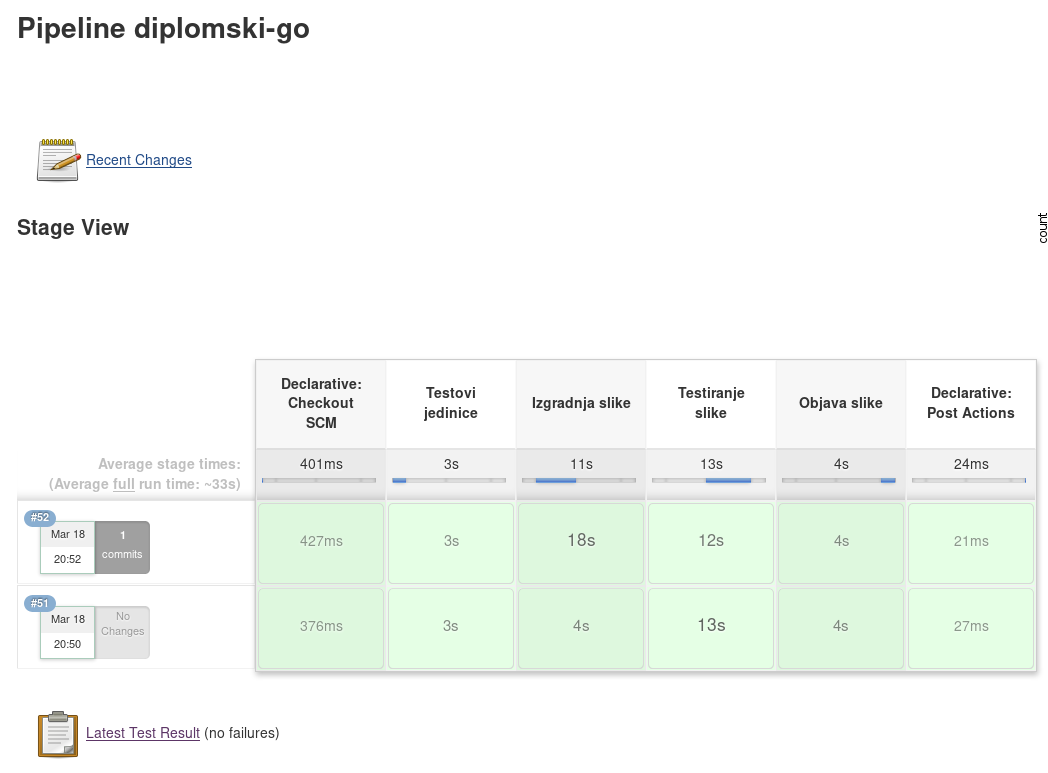
\includegraphics[width=\textwidth]{img/03/jenkins_pipeline.png}
    \caption{Jenkins linija za izgradnju i objavu slike}%
    \label{fig:03jenkins_pipeline}
\end{figure}

Jenkins linija podešena je da periodički provjerava Git projekt, točnije svake minute. Ukoliko je
došlo do promjene u Git projektu, pokreće Jenkins liniju.

U prvoj fazi Jenkins kopira Git projekt koji se poslužuje preko Github servisa. Git projekt javno je
dostupan, stoga nije potrebno podesiti autorizaciju. Nakon što je Git projekt kopiran, Jenkins
uspoređuje razliku između prijašnje i trenutnačne verzije te ih prikazuje korisniku.

U drugoj fazi pokreću se testovi jedinice unutar Docker kontejnera. Fibonacci aplikacija sastoji se
od jednog testa jedinice koji ispituje tri ulaza. Ukoliko dođe do greške, Jenkins linija se prekida.
Pomoću ~\textit{junit} skripte Jenkins objavljuje rezultate testova, kao i vrijeme njihovog
izvođenja.

U trećoj fazi aplikacija se kompajlira i sprema unutar Docker slike. Druga i treća faza dijele istu
baznu Docker sliku. Stoga inženjer može biti siguran da su sve biblioteke dostupne ukoliko su
pokrivene testovima jedinice. Docker slika se označava s trenutnom verzijom izgradnje (\textit{engl.
build number}) te se objavljuje na Docker repositorij. Kako bi se slika mogla objaviti, potrebno je
podesiti Docker autorizaciju unutar Jenkins sustava.

U četvrtoj fazi pokreće se \textit{end-to-end} testiranje pomoću Cypress alata. Jenkins pokreće
Docker kontejner koji pokreće zadnju verziju aplikacije izgrađenu u prethodnom koraku. Zatim u
drugom Docker kontejernu pokreće Cypress alat, koji dalje pokreće testove koji komuniciraju s
novom verzijom aplikacije. Rezultati se objavljuju pomoću \textit{junit} skripte.

U petoj fazi Docker slika se označava sa specijalnom oznakom \textit{latest}. Ta oznaka označava
da je Docker slika spremna za uporabu od strane klijenata. Tu sliku dohvatit će servis za
menadžment.

U zadnjoj fazi, koja se bezuvjetno izvršava, prikupljaju se rezultati testova jedinica i
\textit{end-to-end} testiranja. Rezultati su vidljivi korisniku preko Jenkins web sučelja kao što je
prikazano na slici~\ref{fig:03jenkins_result}.

\begin{figure}[h]
    \centering
    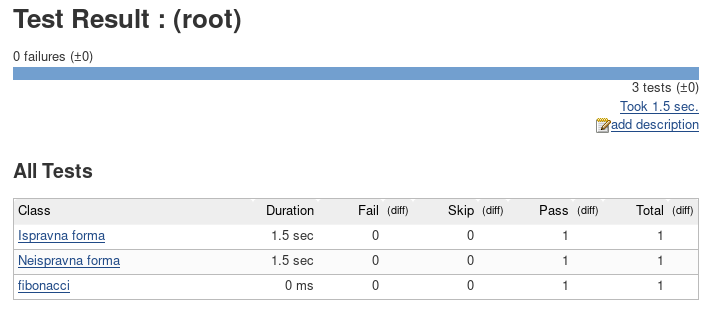
\includegraphics[width=\textwidth]{img/03/jenkins_result.png}
    \caption{Jenkins linija za izgradnju i objavu slike}%
    \label{fig:03jenkins_result}
\end{figure}

\section{Servis za menadžment}
Servis za menadžment je servis zadužen za preuzimanje zadnje Docker slike objavljene na Docker
repositoriju. Prije pokretanja servisa korisnik mora podesiti konfiguracijku datoteku.
Konfiguracijska datoteka je datoteka u \textit{JSON} formatu koja sadrži informacije o Docker slici,
lokaciji Nginx PID datoteci, lokaciji Nginx datotečnoj konfiguracije te vremenu čekanja prilikom
rotiranja verzije aplikacije. Primjer konfiguracije prikazan je kodom~\ref{03jsonconfig}.

\lstset{caption={JSON konfiguracija}, label=03jsonconfig}
\begin{lstlisting}[float=h]
{
    "dockerImage": "sokac/fibonacci",
    "nginxPIDfile": "/run/nginx.pid",
    "nginxConfiguration": "/tmp/nginx.conf",
    "versionOverlapDuration": 30
}

\end{lstlisting}

Informacija o nazivu Docker slike spremljena je pod ključem \texttt{dockerImage}. Servis
zahtjeva da zadnja inačica slike ima oznaku \textit{latest}, što je ujedno i Docker standard.

Nginx PID datoteka, spremljena pod ključem \texttt{nginxPIDfile}, sadrži indentitet Nginx procesa.
Pomoću tog indentiteta moguće je poslati zahtjev Nginx procesu da ponovno učita konfiguracije
datoteke bez prekida posluživanja korisnika.

Nginx datotečna konfiguracija sprema postavke potrebne da Nginx može proslijediti informacije
aplikaciji, to jest Docker kontejneru. Vrijednost je spremljena pod ključem
\texttt{nginxConfiguration}. Primjer generirane konfiguracije prikazan je
kodom~\ref{03nginxconfig}.

\lstset{caption={Nginx konfiguracija}, label=03nginxconfig}
\begin{lstlisting}[float=h]
# Managed by Manager
upstream manager_backend {
    server 127.0.0.1:45105;
}
\end{lstlisting}

\subsection{Arhitektura servisa za menadžment}
Servis za menadžment sastoji se od četiri glavne komponente:
\begin{itemize}
    \item komponenta za konfiguraciju
    \item upravitelj \textit{Unix} signala
    \item dohvatitelj Docker slike
    \item upravitelj Docker slike
\end{itemize}

Komponenta za konfiguraciju zadužena je za učitavanje korisničke \textit{JSON} datoteke te provjeru
njene ispravnosti. Za učitavanje datoteke s tvrdog diska korišten je \texttt{io/ioutil} paket koji
služi za ulazno--izlazne operacije. Kako je konfiguracijska datoteka u \textit{JSON} formatu,
korišten je \texttt{encoding/json} paket koji se nalazi u standardnoj Go biblioteci i baziran je na
standardu \textit{RFC 7159}~\citep{bray2017javascript}. Ukoliko jedna od vrijednosti konfiguracije
nije ispravna, komponenta vraća grešku.

Upravitelj signala je zasebna Go rutina koja čeka dva \textit{Unix} signala: \texttt{SIGINT} i
\texttt{SIGTERM} koji se zaprimaju pomoću specijalnog kanala. Ukoliko servis zaprimi jedan od ta dva
spomenuta signala, započinje s milosrdnim gašenjem servisa pomoću zatvaranja specijalnog kanala.
Upravitelj signala je potreban kako bi sustav mogao biti sigurno ugašen i u trenutku kada je nova
verzija aplikacije objavljena.

Dohvatitelj Docker slike je također zasebna Go rutina. Ova komponenta je zadužena za povremenu
provjeru zadnje Docker slike na udaljenom poslužitelju. Za komunikaciju s Docker servisom koristi
službeni Docker SDK za Go jezik. Komponenta svakih trideset sekundi dohvaća zadnju sliku s
udaljenog poslužitelja te provjerava identifikator Docker slike s prijašnjom verzijom. Ukoliko
postoji izmjena u verziji, tada šalje vrijednost identifikatora u kanal koji se očitava preko
komponente upravitelja Docker slike. Algoritam dohvaćanja nove slike prikazan je
kodom~\ref{03manager_fetcher}.

\lstset{caption={Algoritam dohvatitelja Docker slike}, label=03manager_fetcher}
\begin{lstlisting}[float=h]
func (c *DockerFetcher) fetchLatest() {
	ctx := context.Background()
	defer ctx.Done()

	refStr := fmt.Sprintf("%s:latest", c.image)
	o, err := c.cli.ImagePull(ctx, refStr, types.ImagePullOptions{})
	if o != nil {
		defer o.Close()
	}
	if err != nil {
		log.Println("Couldn't pull the latest image", err.Error())
		return
	}
	inspect, _, err := c.cli.ImageInspectWithRaw(ctx, refStr)
	if err != nil {
		log.Println("Couldn't pull the latest image", err.Error())
		return
	}
	if c.latestID != inspect.ID {
		log.Println("New image found", inspect.ID)
		c.ch <- inspect.ID
		c.latestID = inspect.ID
	}
}
\end{lstlisting}

Komponenta upravitelja Docker slike je isto tako zasebna Go rutina. Za razliku od dohvatitelja, ona
isključivo čeka na poruku od kanala. Kada je identifikator Docker slike zaprimljen kroz kanal,
pokreće se algoritam za pokretanje nove aplikacije. Algoritam prvo mora pronaći slobodan TCP port na
kojem nova aplikacija može slušati, što je prikazano kodom~\ref{03manager_port}. Korištenje
statičkog porta nije moguće jer bi prethodna verzija aplikacija slušala na tom portu. Ukoliko se
stara verzija aplikacija ugasi radi pokretanja nove verzija, tada će takva aplikacija biti nedostupna
onoliko koliko je potrebno da se aplikacija pokrene, što nije prihvatljivo za moderne aplikacije.

\lstset{caption={Algoritam za pronalazak slobodnog porta}, label=03manager_port}
\begin{lstlisting}[float=h]
func getFreePort() (int, error) {
	tcpAddr, err := net.ResolveTCPAddr("tcp", "127.0.0.1:0")
	if err != nil {
		return 0, err
	}
	l, err := net.ListenTCP("tcp", tcpAddr)
	if err != nil {
		return 0, err
	}
	defer l.Close()
	return l.Addr().(*net.TCPAddr).Port, nil
}
\end{lstlisting}

Nakon što je slobodan port pronađen, pokreće se Docker kontejner sa zadnjom verzijom aplikacije.
Kontejner se pokreće u mostovnom mrežnom načinu rada te prosljeđuje zathjeve sa slobodnog porta
glavnog računala prema aplikaciji koja se izvršava unutar Docker kontejnera. Također se zadaje
naredba Docker servisu da obriše sliku po zaustavljanju Docker kontejnera.

Nakon pokretanja Docker kontejnera, obavještavaju se svi pretplatnici. Pretplanik je struktura
opisana \texttt{Subscriber} sučeljem, koji je prikazan kodom~\ref{03manager_subscriber}. Pretplanik
može izvšiti bilo kakvu operaciju nakon što je obavješten, kao što je slanje elekroničke pošte za
novu verziju, slanje \textit{IRC} poruke, promjena konfiguracije web servisa, rotacija log datoteka,
itd.

\lstset{caption={Sučelje pretplatnika}, label=03manager_subscriber}
\begin{lstlisting}[float=h]
type Subscribers interface {
	NewContainer(dockerPort int)
}
\end{lstlisting}

U ovom radu isprogramiran je samo jedan pretplanik - Nginx. Nginx pretplatnik zapisuje novu
konfiguraciju unutar datoteke zadanu konfiguracijom \texttt{nginxConfiguration}. Konfiguracijska
datoteka prikazana je kodom~\ref{03nginxconfig}. Nakon što je datoteka zapisana, učitava se procesni
identifikator nginx procesa preko \textit{PID} datoteke. Zatim se šalje Unix signal \texttt{SIGHUP}
nginx procesu pomoću \texttt{syscall} paketa koji obavještava Nginx da ponovno učita konfiguracijske
datoteke. U tom trenutku Nginx počinje posluživati korisnike s novom aplikacijom.

Nakon što su svi pretplatnici obavješteni i izvršili potprogram, upravitelj Docker slike čeka zadano
vrijeme \texttt{versionOverlapDuration} te zatim gasi stari Docker kontejner. Stari Docker kontejner
prima signal \texttt{SIGTERM} koji omogućava milosrdno gašenje aplikacije. Ukoliko se kontejner ne
ugasi nakon deset sekundi, šalje se \texttt{SIGKILL} koji nasilno gasi aplikaciju i kontejner, koji
se zatim briše.

\subsection{Rad servisa}
Prilikom pokretanja servisa učitava se konfiguracijska datoteka te se provjerava njena ispravnost.
Ukoliko je konfiguracija datoteka neispravna, program ispisuje pogrešku te prekida rad. Ako je
konfiguracijska datoteka ispravna, servis počinje periodički provjeravati izmjene na udaljenom
repositoriju. Ukoliko je došlo do promjene slike s oznakom \textit{latest}, servis pokreće novi
Docker kontejner koji prihvaća zahtjeve na nekorištenom \textit{TCP portu}. Zatim zapisuje novu
Nginx konfiguraciju na tvrdi disk te šalje \textit{SIGHUP Unix} signal Nginx procesu. Takav signal
služi za učitavanje promjena konfiguracije. Nakon korisnički definiranog vremena, stari Docker
kontejner se gasi te automatski briše. Pojednostavljeni dijagram toka prikazan je
slikom~\ref{fig:03servismanagement}.

\begin{figure}[h]
    \centering
    \begin{tikzpicture}[
        scale=1.0,
        node distance=1cm,
        text width=3.5cm,
        text centered,
        block/.style={
            rectangle,
            draw,
            text width=10em,
            text centered,
            rounded corners,
        },
        process/.style={
            rectangle,
            draw,
            text width=10em,
            text centered,
        },
        decision/.style={
            diamond,
            draw,
            text width=4em,
            text badly centered,
            inner sep=0pt,
        },
        arrow/.style={
            thick,->,>=stealth
        },
    ]
        \node [block] (start) {POČETAK};

        \node [process, below=of start] (loadconfig) {Učitaj postavke};

        \node [process, below=of loadconfig] (checkversion) {Provjeri zadnju verziju slike};

        \node [left=of checkversion] (e2) {};

        \node [decision, below=of checkversion] (newversion) {Nova verzija?};

        \node [process, below=of newversion] (launch) {Pokreni najnoviju verziju};
        \node [process, below=of launch] (save) {Spremni novu Nginx konfiguraciju};
        \node [process, below=of save] (reload) {Učitaj Nginx promjene};
        \node [process, below=of reload] (shutdown) {Ugasi stari kontejner};

        \draw [arrow] (start) -- (loadconfig);
        \draw [arrow] (loadconfig) -- (checkversion);
        \draw [arrow] (checkversion) -- (newversion);
        \draw [arrow] (newversion) -- node[anchor=south] {NE} ++(-4.5cm,0cm) |- (checkversion);

        \draw [arrow] (newversion) -- node[xshift=-5mm] {DA} (launch);
        \draw [arrow] (launch) -- (save);
        \draw [arrow] (save) -- (reload);
        \draw [arrow] (reload) -- (shutdown);
        \draw [arrow] (shutdown) -- ++(+4.5cm,0cm) |- (checkversion);
    \end{tikzpicture}
    \caption{Pojednostavljeni dijagram toka servisa za menadžment}%
    \label{fig:03servismanagement}
\end{figure}

Generirana Nginx konfiguracija sadrži samo informacije o Docker kontejeru te kao takva nije potpuna.
Glavna Nginx konfiguracija priključuje takvu konfiguraciju pomoću direktive \texttt{include}.
Primjer glavne Nginx konfiguracije prikazan je kodom~\ref{03nginxconfig2}.

\lstset{caption={Nginx konfiguracija}, label=03nginxconfig2}
\begin{lstlisting}[float=h]
worker_processes 1; # broj radnika

events {
    worker_connections  1024; # broj veza po radniku
}

http {
    include /tmp/nginx.conf; # Lokacija generirane Nginx konfiguracije

    keepalive_timeout  60; # Vrijeme koliko dugo ce veza biti otvorena

    server {
        listen       80; # Port slusanja
        server_name  localhost; # Domena

        location / {
            proxy_pass http://manager_backend; # Proslijedi zahtjev
        }
    }
}
\end{lstlisting}
